% !TEX root = calculus.tex

\chapter{MORE ON THE LIMIT OF FUNCTION}
\label{more-limit-func}
{\parindent=0pt
\rdr Comparing the definition of the limit of a function at a point with the definition of the limit of a numerical sequence, I come to the conclusion that these two limits are of different nature.

\athr And I understand why. In fact, I did emphasize the difference myself in the previous dialogue, pointing out, as you probably remember, that a sequence is a function defined on a set of integers, while the functions we are discussing at the moment are defined over intervals. I doubt, however, that you are justified in speaking about the difference in the nature of the limit of function and that of sequence. In the final analysis (and this is essential) \emph{the limit of a function at a point may be defined on the basis of the limit of a numerical sequence}.

\rdr This is very interesting.

\athr Let us forget, for the time being, about the definition of the limit of function given in the previous dialogue. Consider a new definition.
We shall consider, as before, a function, $f (x)$ defined over an interval, and a point $x = a$ either taken within the interval or coinciding with its end.

\athr The two are \emph{equivalent}. 

\rdr But in form they are quite different.

\athr We can prove their equivalence. To begin with, let the definition using a $\delta$-neighbourhood of point a be called ``definition \emph{1}'', and the definition using numerical sequences, ``definition \emph{2}''.

Now, what two theorems must be proved to demonstrate the equivalence of definitions \emph{1} and \emph{2}? Can you formulate these theorems?

\rdr We have to prove two theorems, one direct and the other converse. We want to prove that definition \emph{2} follows from definition \emph{1} and vice versa (i.e. definition \emph{1} follows from	definition \emph{2}).

\athr Correct. First, I shall prove the following theorem.
\begin{mytheo}{Theorem} If a number $b$ is the limit of a function $f (x)$ at a point $a$, in terms of definition \emph{1}, it is the limit of the function $f (x)$ at $a$ in terms of definition \emph{2} as well.
\end{mytheo}

Since $b$ is the limit of the function $f (x)$ at point a in terms of definition \emph{1} (this is given), consequently, for any $\varepsilon > 0$ there is $\delta > 0$ such that $| f(x)- b | < \varepsilon$  for all $x \neq a$ from a $\delta$-neighbourhood of point $a$. Then we ``construct''	an	arbitrary	sequence	($x_{n}$) ,	requiring	that	it	be convergent to point $a$ (any $x_{n}$ belong to the domain of the function and $x_{n} \neq a$ for any $n$). As a result we obtain a sequence of the corresponding values of the function (the sequence	$[f (x_{n} ) ]$) .	We	want	to	prove	that	the	sequence $[f (x_{n} )]$ is convergent to $b$.

First, I select an arbitrary $\varepsilon > 0$. I should find a number $N$ such that $|f(x_{n}) -	b| < \varepsilon$ for all $n > N$.

I cannot immediately find such $N$ for an arbitrary $\varepsilon$. However, I can indicate for an arbitrary $\varepsilon$ such $\delta$ that $| f(x)- b | < \varepsilon$  
if $|x- a| < \varepsilon$. Then I take this $\delta$ and find a sequence $(x_{n})$ convergent to $a$. Evidently, since $(x_{n})$ is convergent to $a$,  $\varepsilon$(as any other positive real number) can be placed in correspondence with a number $N$ such that $|x_{n} - a| < \delta$ for all $n > N$. And, consequently, we
also have that $|f(x_{n}) - b| < \varepsilon$ for all $n > N$. Hence we find that the thus found number $N$ is actually the desired number.	It proves	the	convergence	of	the	sequence $[f (x_{n} )]$ to	$b$. Since	the sequence	$(x_{n} )$,	which	is	convergent	to	$a$ was chosen (``constructed'') arbitrarily, we conclude that the theorem's proof is completed.

If the line of reasoning is clear to you, try briefly to recapitulate the logical 
structure of the proof.

\begin{figure}[!ht]%[13]{r}{0.5\textwidth}
\centering
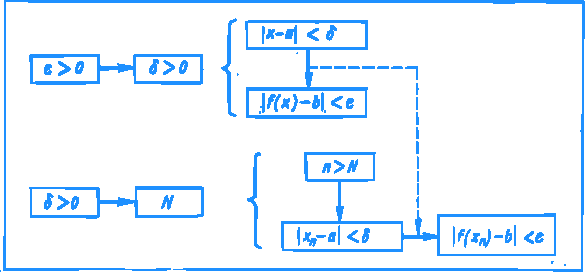
\includegraphics[width=\textwidth]{figures/fig-30.pdf}
\caption{Schematic diagram of the proof that two definitions of the limit of a function are equal.}
\label{fig-30}
\end{figure}

\rdr I shall try to present the structure of the proof as a diagram (\fig{fig-30}).

\athr Your diagram is correct. Will you expand on it. 

\rdr The \emph{first step} of the proof: we find for an arbitrary $\varepsilon
> 0$ a number $\delta > 0$ such that $| f(x)- b | < \varepsilon$ if $|x - a| < \delta$. 

The \emph{second step} of the proof: we take $\delta$ selected at the
first step; choose a sequence $(x_{n})$ convergent to $a$, and find a number $N$ such that  $|x - a| < \delta$ for all $n > N$. Having in mind the arguments used at the first step, we conclude that $| f(x)- b | < \varepsilon$. 

We have thus found for an arbitrary $\varepsilon > 0$ a number $N$ such that  $| f(x_{n})- b | < \varepsilon$ for all $n > N$. This completes the proof.

\athr Correct. In conclusion I want to emphasize several essential points on which the proof hinges. We know that $| f(x)- b | < \varepsilon$ for any $x$ from the $\delta$-neighbourood of $a$. Since a sequence $(x_{n})$ is convergent to $a$, all $x_{n}$ (the whole infinite ``tail'' of the sequence $(x_{n})$ starting from a certain number $N +1$) are contained inside the $\delta$-neighbourhood of point $a$. It then follows that all $f (x_{n} )$ (the whole infinite	``tail'' of the sequence $[f (x_{n} )]$ starting from the same number N + 1.) are contained inside the interval $] b - \varepsilon, b + \varepsilon[$, This proves that the sequence $[f (x_{n})]$ converges to $b$.

\rdr I understand.

\athr Now I am going to prove the following converse theorem.
\begin{mytheo}{Theorem}
If a number $b$ is the limit of a function $f (x)$ at a point $a$ in terms of definition \emph{2}, it is also the limit of the function $f (x)$ at a in terms of definition \emph{1}.
\end{mytheo}
In this case I shall use the proof by contradiction. Assume the contrary to what is to be proved, namely, assume that $b$, the limit of $f (x)$ in terms of definition \emph{2}, is not, however, the limit of $f (x)$ in terms of definition \emph{1}. Can you formulate the last proposition (more exactly, the assumption)?

\rdr As far as I remember, a similar formulation has already been discussed in the previous dialogue. If $b$ is not the limit of the function $f (x)$ at point $a$ (in terms of definition \emph{1}), it means that there is $\varepsilon' > 0$ such that it is impossible to find a necessary $\delta> 0$. Namely, no matter what $\delta$ we select, each time the function $f (x) $assumes a value outside of $]b - \varepsilon', \, b + \varepsilon'[$ for at least one point $x$ from the $\delta$-neighbourhood of point $a$, i.e. the inequality $| f(x)- b | < \varepsilon'$ is violated.

\athr Correct. Assume that we have selected precisely this $ \varepsilon' > 0$. Next take an arbitrary $\delta> 0$, for instance, $\delta_{1} = 1$. As you have said, in any $\delta$-neighbourhood of point $a$ and, hence, in the $\delta$-neighbourhood of this point there is at least one point $x$ (denoted by $x_{1}$) such that $|f(x_{1} -b|  \geqslant \varepsilon'$.

\rdr What happens if the $\delta$-neighbourhood contains many such points $x$? 

\athr It makes no difference. The important fact is that there is \emph{at least one such point}. If there are several such points, take anyone of them and denote it by $x_{1}$.

Now we take a new $\delta$, for instance, $\delta_{2} = \dfrac{1}{2}$. According
to our assumption, the $\delta_{2}$-neighbourhood of point a will contain at least one point $x$ (denoted by $x_{2}$) such that $|f(x_{2} -b | \geqslant \varepsilon'$.

Further we take $\delta_{3} = \dfrac{1}{3}$.The $\delta_{3}$-neighbourhood of point $a$ will also contain at least one point $x$ (point $x_{3}$) such that $|f(x_{3} -b|  \geqslant \varepsilon'$.

We can continue this process for a sequence of the $\delta$-neighbourhoods of point $a$
\begin{equation*}%
\delta_{1} = 1, \,\, \delta_{2} = \dfrac{1}{2}, \,\, \delta_{3} = \dfrac{1}{3}, \,\, \ldots \delta_{n} = \dfrac{1}{n}, \,\, \ldots
\end{equation*}
Note that the $\delta$-neighbourhoods are selected in such a way that the sequence ($\delta_{n}$) converges to zero (is infinitesimal).

If each time we select from each $\delta$-neighbourhood one point $x$ in which $f (x)$ assumes a value outside of the interval $]b- \varepsilon', \, b + \varepsilon'[$, we obtain a sequence composed of points
\begin{equation*}%
x_{1}, \, x_{3}, \, x_{3}, \, \ldots \, x_{n}, \ldots
\end{equation*}
 Since the sequence ($\delta_{n}$) converges to zero, the sequence $(x_{n})$ 
inevitably converges to $a$. A sequence composed of the corresponding	values	of the function	(the sequence	$[f (x_{n} ) ]$ is not convergent to $b$ because for all $n$ we have $|f(x_{n} -b | \geqslant \varepsilon'$. It means that we obtained a sequence $(x_{n} )$ convergent to a for which the sequence $[f (x_{n} ) ]$ is divergent.

This contradicts the condition of the theorem which states that $b$ is the limit of the function at $a$ in terms of definition \emph{2}. It means that for any sequence $(x_{n} )$ convergent to a the corresponding sequence $[f (x_{n} )$  must be convergent to $b$. And the sequence $(x_{n})$ that we have found contradicts this condition.

Hence, the assumption that $b$, being the limit of the function in terms of definition \emph{2}, is not at the same time the limit of the function in terms of definition \emph{1}, is invalidated. This completes the proof of the theorem.

\rdr I must admit of being wrong when I spoke about different natures, of the limit of numerical sequence and the limit of function at a point.

\athr These limits differ but \emph{their nature is the same}. The concept of the \emph{limit of function at a point} is based, as we have seen, on the concept of the \emph{limit of numerical sequence}.

That is why basic theorems about the limits of functions are analogous to those about the limits of sequences.

\rdr We have already noted one of such theorems: the \emph{theorem on the uniqueness of the limit of function at a point}.

\athr This theorem is analogous to that about the uniqueness of the limit of numerical sequence.

I shall also give (without proof) the \emph{theorems on the limit of the sum; the product, and the ratio of functions}.

\begin{mytheo}{Theorems}
If functions $f(x)$ and $g(x)$ have limits at a point $a$, then functions
\begin{equation*}%
\left[f (x) + g (x) \right], \,\, \left[f (x) g (x) \right], \,\, \left( \frac{f(x)}{g(x)} \right)
\end{equation*}
also have limits at this point. These limits equal the sum, product, and ratio, respectively, of the limits of the constituent functions (in the last case it is necessary that the limit of the function $g (x)$ at a be different from zero).
\end{mytheo}
Thus,
\begin{align*}
\lim\limits_{x \to a} [f (x) +g (x)] & = \lim\limits_{x \to a} f (x) + \lim\limits_{x \to a} g (x)\\[5pt]
\lim\limits_{x \to a} [f(x) \, g(x)]& = \lim\limits_{x \to a} f(x) \, \lim\limits_{x \to a} g(x)\\[5pt]
\lim\limits_{x \to a} \left( \frac{f(x)}{g(x)} \right) & = \frac{\lim\limits_{x \to a} f(x)}{\lim\limits_{x \to a} g(x)} \\[5pt]
& \text{under an additional condition} \,\, \lim\limits_{x \to a} g(x) \neq 0
\end{align*}
\rdr We have already discussed the similar theorems for numerical sequences.

\athr Next I wish to make two remarks, using for the purpose specially selected examples.

\textcolor{IndianRed}{\textbf{Note 1.}} It is illustrated by the following example. Obviously
\begin{equation*}%
 \lim\limits_{x \to a} \sqrt{1 - x^{2}} = 0 \,\, \text{and} \,\,  \lim\limits_{x \to a} \sqrt{x - 1} = 0.
  \end{equation*}
  Does it mean that  $\lim\limits_{x \to a} ( \sqrt{1 - x^{2}} + \sqrt{x - 1}) = 0$? 

\rdr The limit of the function $\sqrt{1 - x^{2}}$ at $x = 1$ exists and is equal to zero. The limit of the function $\sqrt{x - 1}$ at $x = 1$ also exists and is also equal to zero. According to the theorem on the limit of the sum, the limit of $f (x) = \sqrt{1 - x^{2}} + \sqrt{x - 1}$ must exist and be equal to the
sum of the two preceding limits, i.e. to zero.

\athr Nevertheless, $f (x) = \sqrt{1 - x^{2}} + \sqrt{x - 1}$ no limit at $x = 1$ for a simple reason that the expression $\sqrt{1 - x^{2}} + \sqrt{x - 1}$ has meaning only at a single point (point $x = 1$). Applying the theorem on the limit of the sum, you have not taken into account the domains of the functions  $\sqrt{1 - x^{2}}$ and  $ \sqrt{x - 1}$. The former has the natural domain over $[-1, \,1]$, while the latter over $[1, \infty[$. 

\rdr Apparently your note also covers the cases when the theorems on the limit of the product and the limit of the ratio of functions are used.

\athr It goes without saying. Working with functions, you must always consider their domains. The natural domains of functions may intersect (or even coincide), but sometimes they may not. This aspect must never be over-looked. Why do you think we never have such complications when working with sequences?

\rdr Obviously because all numerical sequences have one and the same domain, i.e. a set of natural numbers. 

\athr Correct. Now we come to 

\textcolor{IndianRed}{\textbf{Note 2}}. Do you think the limit
\begin{equation*}%
  \lim\limits_{x \to 0} \, \frac{\sin x}{x} \,\, \text{exists?}
  \end{equation*}
  
\rdr In any case the theorem on the limit of the ratio is not valid here because  $\lim\limits_{x \to 0} x = 0$.

\athr In fact, if $\lim\limits_{x \to 0} f(x) = 0$ and $\lim\limits_{x \to 0} g(x) = 0$, the limit of their ratio i.e., the limit of the function $ \dfrac{f(x)}{g(x)}$
may exist. 

\rdr What is this limit? 

\athr It depends on the functions $f(x)$ and $g (x)$.
Let us show, for example, that 
\begin{equation*}%
\boxed{  \lim\limits_{x \to 0} \, \frac{\sin x}{x}  = 1}
\end{equation*}
Note that the function $\dfrac{\sin x}{x} $ is not defined at $x = 0$. This
fact, however, does not interfere with searching for the limit of the function at $x = 0$.

We shall start with well-known inequalities: 
\begin{equation*}%
\sin x < x < \tan x	\,\, \left( 0 < x < \frac{\pi}{2} \right)
\end{equation*}

An assumption that $\left( 0 < x < \frac{\pi}{2} \right)$ will not affect the generality of our results. Dividing $\sin x$ by each term of these inequalities, we obtain 
\begin{equation*}%
1 >   \frac{\sin x}{x}   > \cos x
\end{equation*}
hence
\begin{equation*}%
0 <  \left( 1-  \frac{\sin x}{x}  \right)  < ( 1 -  \cos x)
\end{equation*}
Next we take into account that
\begin{equation*}%
 1 -  \cos x = 2 \sin^{2} \dfrac{x}{2} < 2 \sin \dfrac{x}{2} < 2 \dfrac{x}{2} = x
\end{equation*}
Thus we have
\begin{equation*}%
0 <  \left( 1-  \frac{\sin x}{x}  \right)  < x
\end{equation*}
or 
\begin{equation*}%
-x  <  - \left( 1-  \frac{\sin x}{x}  \right)  < 0
\end{equation*}
whence
\begin{equation*}%
 \left|1 - \frac{\sin x}{x} \right|  < |x|
\end{equation*}
We thus arrive at the following inequality valid for $ |x| < \frac{\pi}{2} $
\begin{equation}%
 \left| \frac{\sin x}{x}  -1 \right|  < |x|
 \label{sinc-limit}
 %eq-1
\end{equation}
By using this inequality, we can easily prove that the
function $\dfrac{\sin x}{x}$ has the limit at $x = 0$, and this limit is
unity. It will be convenient to use definition \emph{1} for the limit of function at a point.

Select an arbitrary $\varepsilon > 0$, demanding for the sake of
simplicity that $\varepsilon < \dfrac{\pi}{2}$. For $\delta$, it is sufficient to take $\delta  =	\varepsilon$  since, according to \eqref{sinc-limit}, the condition $| x - 0 | < \delta$ immediately leads to
\begin{equation*}%
 \left| \frac{\sin x}{x} - 1 \right|  < \delta = \varepsilon
\end{equation*}
Thus, unity is indeed the limit of the function $ \dfrac{\sin x}{x}$ at
$x = 0$. 

\rdr Do we really have to resort to a similar line
of reasoning, based on the definition of the limit of function
at a point, each time we have to find the limit of $ \dfrac{f(x)}{g(x)}$
when both $\lim\limits_{x \to 0} f(x) = 0$ and $\lim\limits_{x \to 0} g(x) = 0$.

\athr No, of course not. The situation we are speaking about is known as an \emph{indeterminate form} of the type $\dfrac{0}{0}$. There are rules which enable one to analyze such a situation in a relatively straightforward manner and, so to say, ``resolve the indeterminacy''. In practice it is usually not difficult to solve the problem of existence of the limit of a function $ \dfrac{f(x)}{g(x)}$ at a specific point and find its value (if it exists). A few rules of evaluation of indeterminate forms of the type $\dfrac{0}{0}$ (and other types as well) will be discussed later. A systematic analysis of such rules, however, goes beyond the scope of our dialogues.

It is important to stress here the following principle (which is significant for further considerations): although the theorem on the limit of the ratio is not valid in the cases when $\lim\limits_{x \to 0} g(x) = 0$, the limit of a function  $\dfrac{f(x)}{g(x)}$ at a point a may exist if $\lim\limits_{x \to 0} f(x) = 0$. The example of the limit of the function  $ \dfrac{\sin x}{x}$ at $x = 0$  is a convincing
illustration of this principle.

\rdr Presumably, a similar situation may take place for numerical sequences as well?

\athr It certainly may. Here is a simple example: 
\begin{align*}%
(x_{n}) & = 1, \, \frac{1}{8}, \, \frac{1}{27}, \,\frac{1}{64}, \, \ldots \frac{1}{n^{3}}, \, \ldots \quad (\lim\limits_{n \to \infty} x_{n} = 0) \\
(y_{n}) & = 1, \, \frac{1}{2}, \, \frac{1}{3}, \,\frac{1}{4}, \, \ldots \frac{1}{n}, \, \ldots \quad (\lim\limits_{n \to \infty} y_{n} = 0)
\end{align*}
It is readily apparent that the limit of the sequence $ \left(\dfrac{x_{n}}{y_{n}}\right)$ is the limit of the sequence $ \left(\dfrac{1}{n^{2}}\right)$. This limit does exist and is equal to zero.

\rdr You mentioned that the existence of the limit of a function $ \dfrac{f(x)}{g(x)}$ at $a$, when both  $\lim\limits_{x \to 0} f(x) = 0$ and $\lim\limits_{x \to 0} g(x) = 0$ the existence of the limit of the type $\dfrac{0}{0}$, is very important for further considerations. Why? 

\athr The point is that one of the most important concepts in calculus, namely, that of \emph{derivative}, is based on the limit of the type $\dfrac{0}{0}$. This will be clear in the subsequent dialogues.
}